\documentclass{standalone}
\usepackage[landscape]{geometry}
\usepackage{tikz}
\usepackage{pgfplots}
\pgfplotsset{compat=newest}
\usepackage{mathptmx}
\usetikzlibrary{calc,patterns,decorations.pathmorphing,decorations.markings,matrix,fit,decorations.pathreplacing,arrows.meta,automata,positioning,shapes,chains,spy}
\usetikzlibrary{intersections,through,backgrounds}
\usetikzlibrary{shadows,fadings}
% \usepackage[active,tightpage,pdftex]{preview}
% \PreviewEnvironment{tikzpicture}
\definecolor{startColor}{HTML}{D23AD0}
\definecolor{generateColor}{HTML}{833EC3}
\definecolor{doAcceptColor}{HTML}{2B6BD1}
\definecolor{isMaxTriesColor}{HTML}{0BBFCE}
\definecolor{decreaseTempColor}{HTML}{58BD1B}
\definecolor{isMinTempColor}{HTML}{FED02F}
\definecolor{stopColor}{HTML}{F45E30}
\definecolor{replaceColor}{HTML}{E81E49}
\begin{document}
  \large
  \centerline{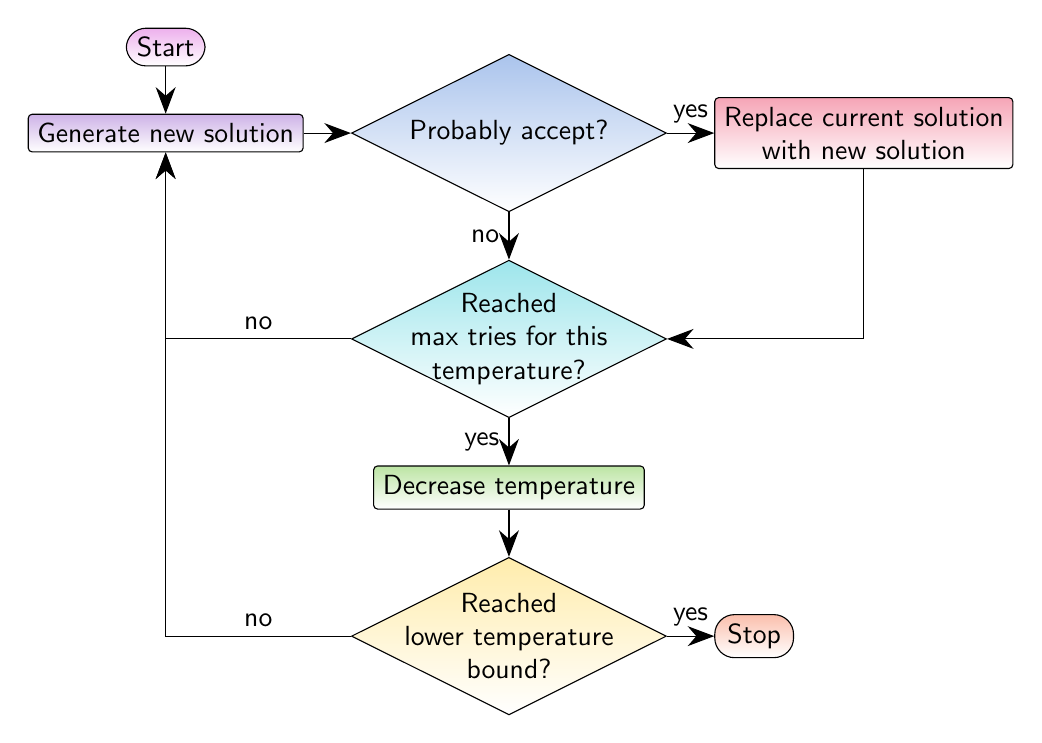
\begin{tikzpicture}[%
    >={Stealth[scale=2.0]},align=center,every node/.style={font=\sffamily}]
    \tikzstyle{base}=[node distance=0.6cm,fill=white,draw=black]
    \tikzstyle{extreme}=[base,text centered,rectangle,rounded corners=0.25cm,minimum width=1.0cm,minimum height=0.45cm]
    \tikzstyle{action}=[base,text centered,rectangle,rounded corners=0.05cm,minimum width=1.0cm,minimum height=0.45cm]
    \tikzstyle{condition}=[base,diamond,aspect=2,text width=10em,inner sep=-12pt,text badly centered,minimum width=4.0cm,minimum height=2cm]
    % All state styles
    \tikzstyle{start}=[extreme,top color=startColor!40]
    \tikzstyle{generate}=[action,top color=generateColor!40]
    \tikzstyle{doAccept}=[condition,top color=doAcceptColor!40]
    \tikzstyle{isMaxTries}=[condition,top color=isMaxTriesColor!40]
    \tikzstyle{decreaseTemp}=[action,top color=decreaseTempColor!40]
    \tikzstyle{isMinTemp}=[condition,top color=isMinTempColor!40]
    \tikzstyle{stop}=[extreme,top color=stopColor!40]
    \tikzstyle{replace}=[action,top color=replaceColor!40]
    % All states
    \node (start) [start]                                    {Start};
    \node (generate) [generate,below=of start]
          {Generate new solution};
    \node (doAccept) [doAccept,right=of generate]
          {Probably accept?};
    \node (isMaxTries) [isMaxTries,below=of doAccept]
          {Reached\\max tries for this\\temperature?};
    \node (decreaseTemp) [decreaseTemp,below=of isMaxTries]
          {Decrease temperature};
    \node (isMinTemp) [isMinTemp,below=of decreaseTemp]
          {Reached\\lower temperature\\bound?};
    \node (replace) [replace,right=of doAccept]
          {Replace current solution\\with new solution};
    \node (stop) [stop,right=of isMinTemp]                   {Stop};
    % Edges
    \draw [->] (start) -- (generate);
    \draw [->] (generate) -- (doAccept);
    \draw [->] (doAccept) -- node[anchor=east] {no} (isMaxTries);
    \draw [->] (doAccept) -- node[anchor=south] {yes} (replace);
    \draw [->] (isMaxTries) -- node[anchor=east] {yes} (decreaseTemp);
    \draw [->] (decreaseTemp) -- (isMinTemp);
    \draw [->] (isMinTemp) -- node[anchor=south] {yes} (stop);
    \draw [->] (replace) |- (isMaxTries);
    \draw [->] (isMaxTries) -| node[anchor=south,near start] {no} (generate);
    \draw [->] (isMinTemp) -| node[anchor=south,near start] {no} (generate);
  \end{tikzpicture}}
\end{document}
